\begin{frame}[allowframebreaks]{Annexes} {Contexte}

    \begin{block}{Paradigme des Systèmes Multi-Agents (SMA) pour des problèmes complexes et distribués}
        \begin{itemize}
            \item \textbf{décomposition des tâches} : missions déléguées aux agents réalisées par coopération~\parencite{Raileanu2023} ;
            \item \textbf{avantages} : gérer des objectifs contradictoires, calcul parallèle, robustesse du système, évolutivité\dots
        \end{itemize}
    \end{block}
    
    \begin{block}{\textbf{Organisation} : clé pour la conception des SMA}
        \begin{itemize}
            \item \textbf{coordination} : comment atteindre un objectif commun de manière collaborative~\parencite{Hubner2007} ;
            \item \textbf{environnements dynamiques et incertains} : comportement flexible à l'exécution pour s'adapter~\parencite{Kathleen2020} ;
        \end{itemize}
    \end{block}
    
    \begin{block}{Méthodes et pratiques pour la conception des SMA}
        \begin{itemize}
            \item \textbf{approche + modèle organisationnel} : les méthodes s'appuient sur l'expérience des concepteurs pour concevoir manuellement les \textbf{politiques} des agents afin que le SMA atteigne ses objectifs ;
                  %   \begin{itemize}
                  %       \item Exemples : \emph{GAIA}~\parencite{Wooldridge2000,Cernuzzi2014}, \emph{ADELFE}~\parencite{Mefteh2015}, ou \emph{DIAMOND}~\parencite{Jamont2015}, \emph{KB-ORG}~\parencite{Sims2008}
                  %   \end{itemize}
            \item \textbf{simulation vers la réalité} : 1) conception sûre et efficace des SMA dans un environnement simulé à haute fidélité ; \quad 2) transfert à un environnement réel pour des performances adéquates~\parencite{Schon2021}.
        \end{itemize}
        \quad $\Longrightarrow$ \textbf{Processus itératif par essais et erreurs}
    \end{block}

\end{frame}

\begin{frame}[allowframebreaks]{Annexes} {Fondamentaux des SMA}

    \begin{block}{Mots-clés}
        \begin{itemize}
            \item \textbf{Agent} : entité immergée dans un environnement, percevant des observations et prenant des décisions de manière autonome pour atteindre des objectifs ;
            \item \textbf{SMA} : ensemble d'agents collaborant avec des mécanismes d'auto/réorganisation pour atteindre leurs objectifs ;
            \item \textbf{Organisation} : interactions des agents même si elles peuvent être implicites ;
            \item \textbf{Modèle organisationnel (OM)} : moyen de décrire formellement une organisation explicite/implicite ;
            \item \textbf{Spécifications organisationnelles (OS)} : composants d'un OM pour caractériser une organisation.
        \end{itemize}
    \end{block}
    
    \begin{block}{Modèle organisationnel : $\mathcal{M}OISE^+$}
        \begin{itemize}
            \item plus complexe que \emph{Agent Group Roles} (intégration des normes) ;
            \item prend explicitement en compte les aspects sociaux entre les agents ;
            \item permet de lier les politiques des agents aux spécifications organisationnelles.
        \end{itemize}
    \end{block}

\end{frame}

\begin{frame}[allowframebreaks]{Annexes} {Fondamentaux du MARL}

    \begin{block}{Mots-clés}
        \begin{itemize}
            \item \textbf{Politique} : la \textquote{logique} pour choisir la prochaine action en fonction de l'observation pour un agent ;
            \item \textbf{Historique/trajectoire} : le couple (observation, action) sur un épisode ;
            \item \textbf{Politique/historique conjoints} : l'ensemble des politiques/historiques de tous les agents sous forme de tuples ;
            \item \textbf{Apprentissage par renforcement} : un agent met à jour sa politique pour maximiser une récompense cumulative ;
            \item \textbf{Apprentissage par renforcement multi-agent (MARL)} : extension à plusieurs agents qui apprennent en prenant en compte les actions des autres agents ;
        \end{itemize}
    \end{block}
    
\end{frame}

\begin{frame}[allowframebreaks]{Annexes}{Approche AOMEA : Fondement théorique}
    \begin{block}{MARL orienté organisation (OMARL)}
        Un processus de MARL augmenté avec un OM pour :
        \begin{itemize}
            \item \textbf{Contraindre l'espace des politiques} : obtenir les politiques conjointes satisfaisant les spécifications de conception données ;
            \item \textbf{Inférer des spécifications organisationnelles} : obtenir des spécifications à partir des politiques des agents.
        \end{itemize}
    \end{block}
    
    \begin{block}{Algorithme \emph{Partial Relations with Agent History and Organization Model} (PRAHOM)}
        Implémentation d'un processus OMARL\dots
        \begin{enumerate}
            \item \textbf{Contraindre l'espace des politiques}
                  \begin{itemize}
                      \item Impossible d'utiliser directement les politiques $\rightarrow$ \textbf{historiques} caractérisant les \textbf{politiques} ;
                      \item Relations entre \textbf{OS} et historiques attendus ;
                      \item Les agents contraints aux OS $\rightarrow$ à chaque étape : actions disponibles mises à jour en fonction des historiques \textbf{OS}.
                  \end{itemize}
    
            \item \textbf{Inférer des spécifications organisationnelles}
                  \begin{itemize}
                      \item Analyser les historiques $\rightarrow$ caractériser les comportements collectifs comme OS ;
                      \item Utilisation des relations connues entre OS et historiques ;
                      \item Utilisation de la définition générale des OS par rapport aux historiques.
                  \end{itemize}
        \end{enumerate}
    \end{block}
    
\end{frame}

\begin{frame}[allowframebreaks]{Annexes}{Approche AOMEA : Fondement théorique}
    \textbf{Contraindre l'espace des politiques} pendant l'entraînement

    \begin{columns}
    
        \begin{column}{0.3\textwidth}
    
            \begin{itemize}
                \item À chaque étape, l'ensemble des actions disponibles est modifié pour correspondre aux contraintes de politiques définies par les utilisateurs ;
                \item Contraintes intégrées via : correction externe, apprentissage, modification interne des politiques.
            \end{itemize}
    
        \end{column}
    
        \begin{column}{0.8\textwidth}
            \begin{figure}
                \centering
                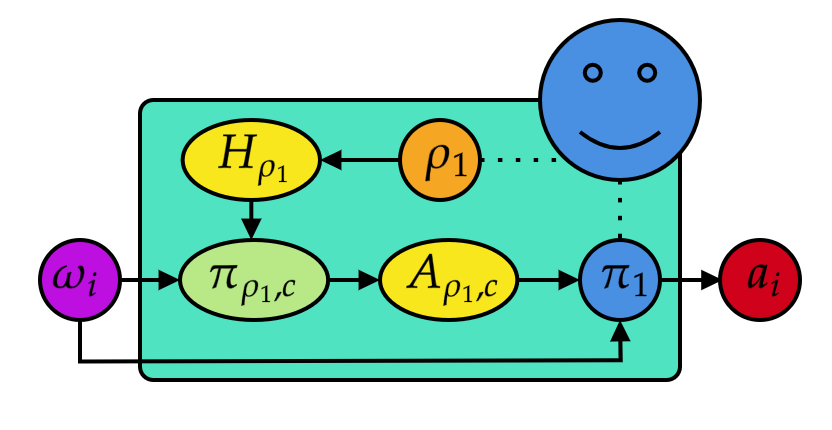
\includegraphics[width=0.7\linewidth]{figures/prahom_training_constrain.png}
                \caption*{Vue résumée de la contrainte PRAHOM}
                \label{fig:prahom_process}
            \end{figure}
        \end{column}
    
    \end{columns}
\end{frame}
    

\begin{frame}[allowframebreaks]{Annexes}{Approche AOMEA: Fondement théorique}

    \textbf{Inferrer des Spécifications Organisationnelles}

    \begin{columns}

        \begin{column}{0.3\textwidth}

            \begin{itemize}
                \item \textbf{Knowledge-based Organizational Specifications Identification (KOSIA)}
                \item \textbf{General Organizational Specifications Infererence (GOSIA)}
            \end{itemize}

        \end{column}

        \begin{column}{0.8\textwidth}
            \begin{figure}
                \centering
                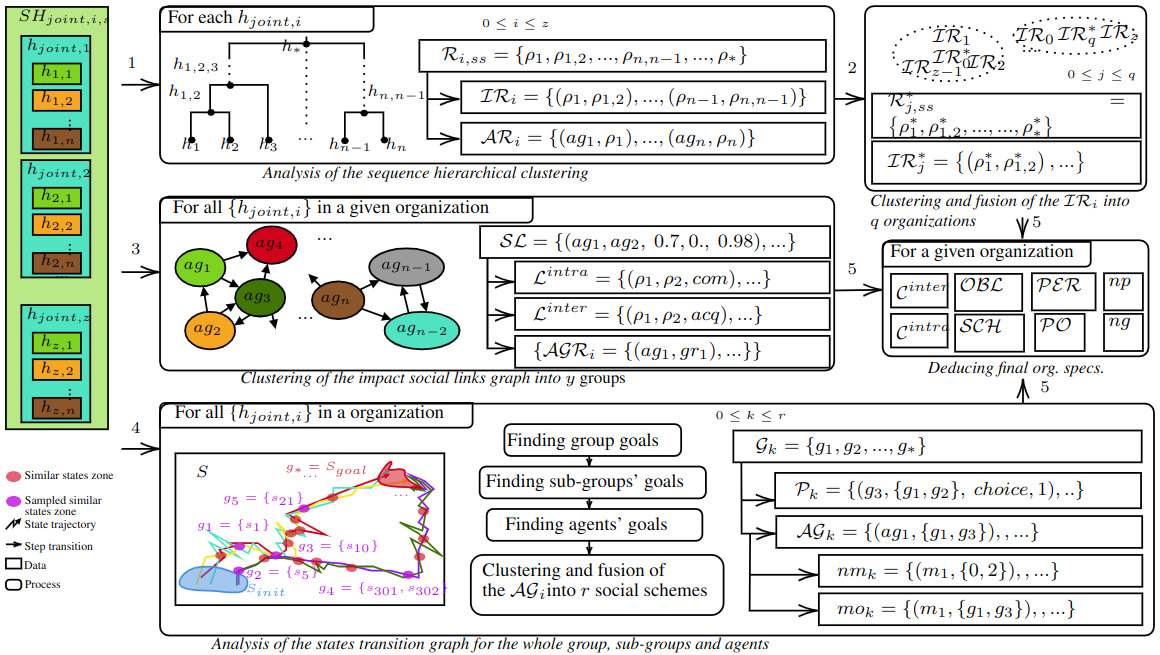
\includegraphics[width=0.95\linewidth]{figures/GOSIA_view.png}
                \caption*{A summary view of the GOSIA process}
                \label{fig:gosia_process}
            \end{figure}
        \end{column}

    \end{columns}

\end{frame}
